% this is my LATEX template file

\documentclass[a4paper]{article}
\usepackage{amssymb,amsmath} 			%for math symbols and etc 
\usepackage{graphicx}       				 %for graphics 
\usepackage{float}  				 	%for float graphics, i.e. , I can place graphics how I want


% title
\title{\textbf{I am changing the title}}
% author
\author{Aleksandar Haber}

\begin{document}

%\def\thefootnote{\fnsymbol{footnote}}
																			\maketitle
\begin{abstract}
This is the abstract. Briefly describe the contents of this report. I am expanding the abstract.
\end{abstract}

\section{Section 1}


This is section 1. In this section we will include mathematical formulas. 
\begin{equation}
E=mc^2
\label{eq2}
\end{equation}

\begin{equation}
x=\frac{y}{z}
\label{eq1}
\end{equation}

In \eqref{eq1} we give our first formula. 

% uncomment this if you need a table of contents 
%\tableofcontents

\begin{align}
 & x = yz  \label{eq1align}  \\
 &  t +t^2+t^3+\frac{t}{\sqrt{t}} =ur  \label{eq2align}
\end{align}

In \eqref{eq1align} and \eqref{eq2align}

Powers:

\begin{align}
x^{3},  x^{y^{z}}
\end{align}

Roots

\begin{align}
\sqrt{x}
\end{align}

Fractions

\begin{align}
\frac{x^{2}}{\sqrt{y}}
\end{align}

Integrals

\begin{align}
\int_{x=0}^{x=5}   d\text{x}
\end{align}

Sums 

\begin{align}
\sum_{i=0}^{i=5} x_{i}
\end{align}

\begin{align}
m\vec{a}=\vec{F}
\end{align}

Dots, derivatives

\begin{align}
\ddot{x}
\end{align}

vectors

\begin{align}
A= \begin{bmatrix} a_{11} & a_{12} \\ a_{21} & a_{22} \end{bmatrix}
\end{align}


Tables


\begin{table}[H]
\begin{center}
  \begin{tabular}{ | l ||| c || r ||}
    \hline
    1 & 2 & 3 \\ \hline
    4 & 5 & 6 \\ \hline 
    7 & 8 & 9 \\
    \hline
  \end{tabular}
\end{center}
\caption{This table presents the measurements results}
\label{Table1}
\end{table}

Go to the next page 

\newpage
Figures

\begin{figure}[H]
\centering
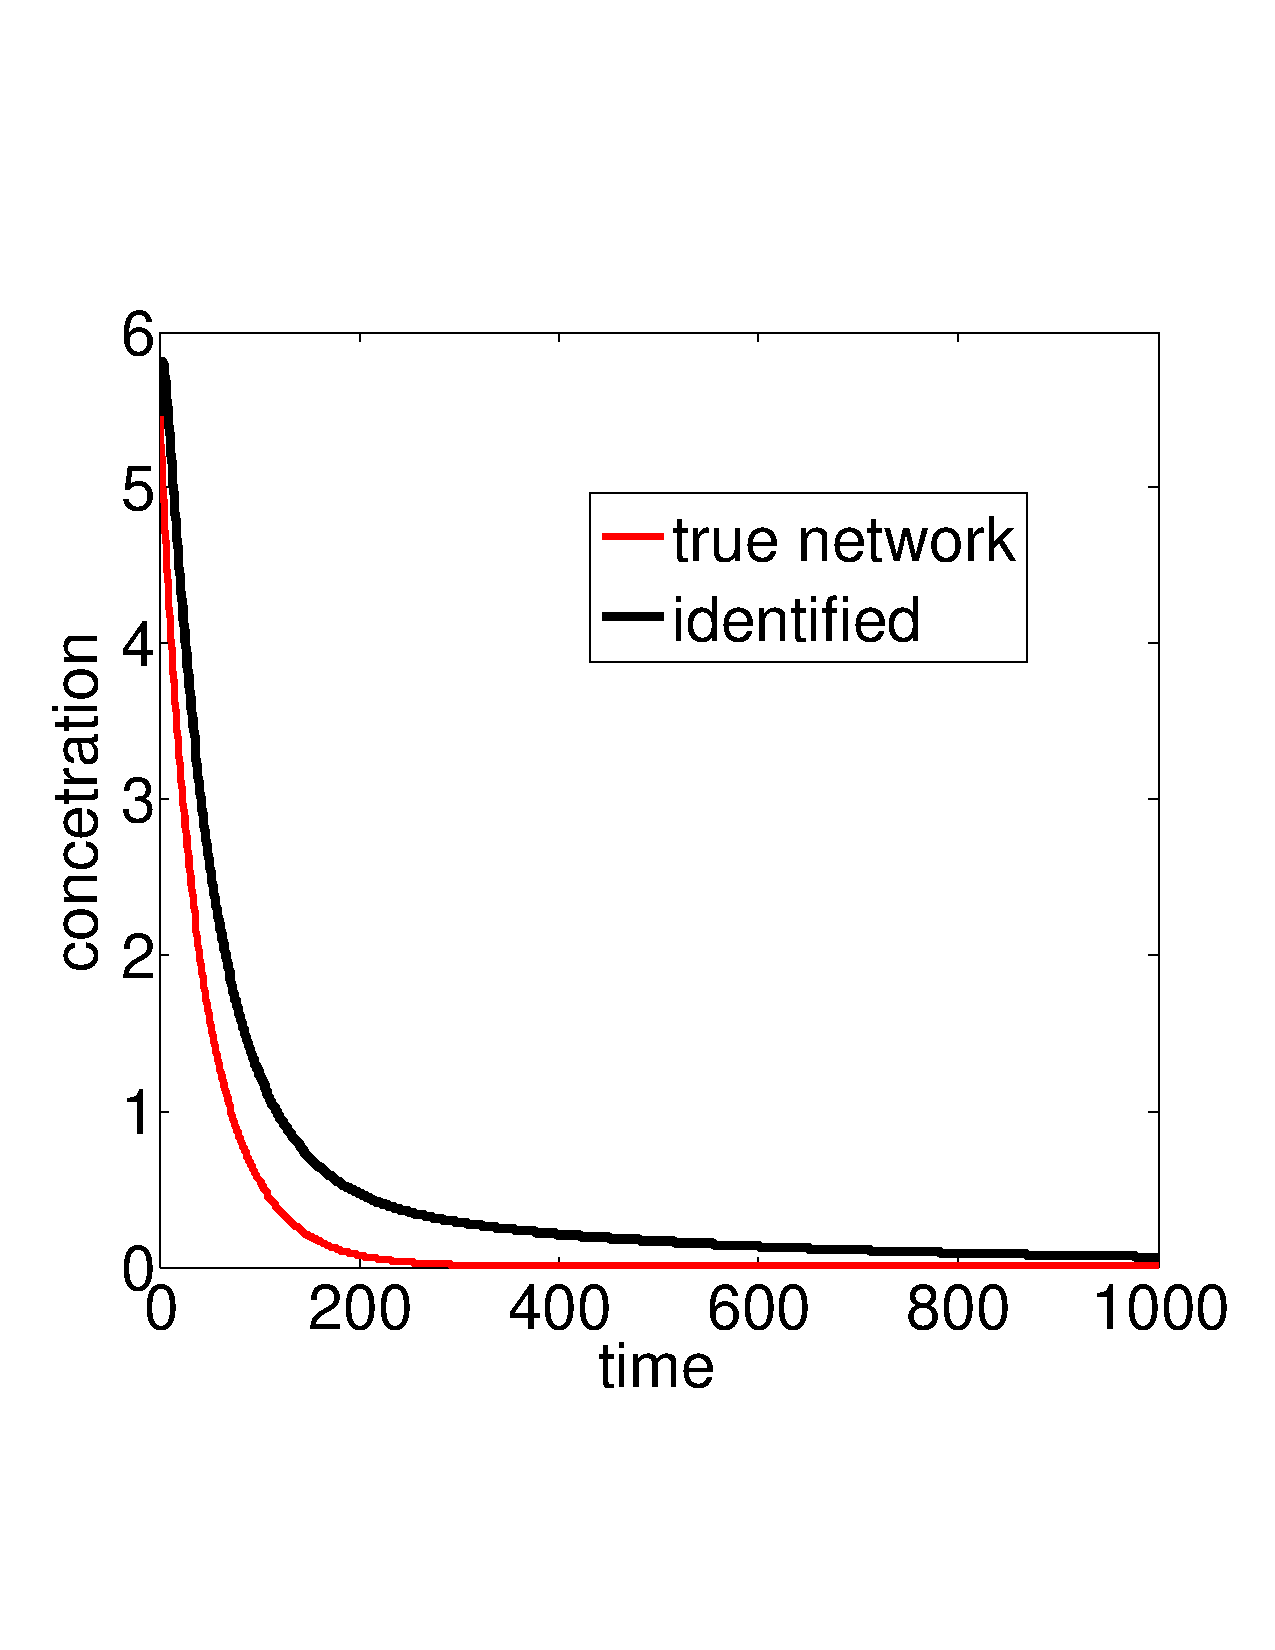
\includegraphics[scale=0.3]{fig2}
\caption{This figure shows a decaying function. Another caption}
\label{label_fig}
\end{figure}

in Fig.~\ref{label_fig}

In the book of Einstein  \cite{einstein1979general}



\bibliographystyle{unsrt}
\bibliography{bibl}


\end{document}


